\documentclass[10pt]{article}
\usepackage[OE]{express}

\begin{document}
\title{Simple model for ring resonators backscatter}
\author{Joaquin Matres and Wayne V. Sorin}  
\address{Hewlett Packard Labs, 1501 Page Mill Road, Palo Alto, CA 94304, USA} 
\email{*wayne.sorin@hpe.com} 


\begin{abstract}
Waveguide backscatter affects the resonance shape and quality factor (Q) of ring resonators.
Our simple analytical expression predicts how waveguide backscatter spoils the Q and results in resonance splitting.
We show that the effects of backscatter depend only on the finesse of the resonator and when it can safely be ignored.
Finally, we describe the effects of backscatter in low-loss cavities using simple complex Lorentzian functions.
\end{abstract}

\ocis{(130.0130) Integrated optics, (290.1350) Backscattering, (230.5750) Resonators.}
%https://www.osapublishing.org/oe/submit/ocis/

%%%%%%%%%%%%%%%%%%%%%%% References %%%%%%%%%%%%%%%%%%%%%%%%%
\begin{thebibliography}{10}
\newcommand{\enquote}[1]{``#1''}

\bibitem{Little1997a}
B.~E. Little, S.~T. Chu, H.~A. Haus, J.~Foresi, and J.~Laine,
  \enquote{{Microring resonator channel dropping filter},} J. Light. Technol.
  \textbf{15}, 998--1005 (1997).

\bibitem{Bogaerts:12}
W.~Bogaerts, P.~{De Heyn}, T.~{Van Vaerenbergh}, K.~{De Vos}, S.~{Kumar
  Selvaraja}, T.~Claes, P.~Dumon, P.~Bienstman, D.~{Van Thourhout}, and
  R.~Baets, \enquote{{Silicon microring resonators},} Laser Photon. Rev.
  \textbf{6}, 47--73 (2012).

\bibitem{Weiss:95}
D.~S. Weiss, V.~Sandoghdar, J.~Hare, V.~Lef{\`{e}}vre-Seguin, J.-M. Raimond,
  and S.~Haroche, \enquote{{Splitting of high-Q Mie modes induced by light
  backscattering in silica microspheres},} Opt. Lett. \textbf{20}, 1835--1837
  (1995).

\bibitem{PhysRevLett.99.173603}
A.~Mazzei, S.~G{\"{o}}tzinger, L.~{de S. Menezes}, G.~Zumofen, O.~Benson, and
  V.~Sandoghdar, \enquote{{Controlled Coupling of Counterpropagating
  Whispering-Gallery Modes by a Single Rayleigh Scatterer: A Classical Problem
  in a Quantum Optical Light},} Phys. Rev. Lett. \textbf{99}, 173603 (2007).

\bibitem{Little1997}
B.~E. Little, J.~P. Laine, and S.~T. Chu, \enquote{{Surface-roughness-induced
  contradirectional coupling in ring and disk resonators.}} Opt. Lett.
  \textbf{22}, 4--6 (1997).

\bibitem{Borselli2004}
M.~Borselli, K.~Srinivasan, P.~E. Barclay, and O.~Painter, \enquote{{Rayleigh
  scattering, mode coupling, and optical loss in silicon microdisks},} Appl.
  Phys. Lett. \textbf{85}, 3693--3695 (2004).

\bibitem{Canciamilla2009}
A.~Canciamilla, M.~Torreggiani, C.~Ferrari, F.~Morichetti, R.~Costa, and
  A.~Melloni, \enquote{{Backscatter in integrated optical waveguides and
  circuits},} Proc. SPIE \textbf{7218}, 72180N--72180N--11 (2009).

\bibitem{Morichetti2010c}
F.~Morichetti, A.~Canciamilla, M.~Martinelli, A.~Samarelli, R.~M. {De La Rue},
  M.~Sorel, and A.~Melloni, \enquote{{Coherent backscattering in optical
  microring resonators},} Appl. Phys. Lett. \textbf{96}, 081112 (2010).

\bibitem{Ballesteros2011}
G.~Ballesteros, J.~Matres, J.~Mart{\'{i}}, and C.~Oton,
  \enquote{{Characterizing and modeling backscattering in silicon microring
  resonators},} Opt. Express \textbf{1005} (2011).

\bibitem{Li2016}
A.~Li, T.~{Van Vaerenbergh}, P.~{De Heyn}, P.~Bienstman, and W.~Bogaerts,
  \enquote{{Backscattering in silicon microring resonators: a quantitative
  analysis},} Laser Photon. Rev. \textbf{10}, 420--431 (2016).

\bibitem{Siegman1986}
A.~E. Siegman, \enquote{{Lasers}} Univ. Sci.~books (1986).

\bibitem{Shi:07}
Z.~Shi, R.~W. Boyd, D.~J. Gauthier, and C.~C. Dudley, \enquote{{Enhancing the
  spectral sensitivity of interferometers using slow-light media},} Opt. Lett.
  \textbf{32}, 915--917 (2007).

\bibitem{Melloni2010}
A.~Melloni, A.~Canciamilla, C.~Ferrari, F.~Morichetti, L.~O'Faolain, T.~F.
  Krauss, R.~{De La Rue}, A.~Samarelli, and M.~Sorel, \enquote{{Tunable delay
  lines in silicon photonics: Coupled resonators and photonic crystals, a
  comparison},} IEEE Photonics J. \textbf{2}, 181--194 (2010).

\bibitem{Melati2014a}
D.~Melati, A.~Melloni, and F.~Morichetti, \enquote{{Real photonic waveguides:
  guiding light through imperfections},} Adv. Opt. Photonics \textbf{6}, 156
  (2014).

\bibitem{Bojko2011}
R.~J. Bojko, J.~Li, L.~He, T.~Baehr-Jones, M.~Hochberg, and Y.~Aida,
  \enquote{{Electron beam lithography writing strategies for low loss, high
  confinement silicon optical waveguides},} J. Vac. Sci. Technol. B
  Microelectron. Nanom. Struct. \textbf{29}, 06F309 (2011).
\end{thebibliography}

%\bibliographystyle{osajnl}
%\bibliography{/Users/joaquin/Dropbox/library}

%%%%%%%%%%%%%%%%%%%%%%%%%%  body  %%%%%%%%%%%%%%%%%%%%%%%%%%
\section{Introduction}
Integrated waveguide optics offers the potential for small, low-cost and high performance optical systems that can be used for high volume communications and sensing.
Optical resonators, such as ring cavities, are a key building block in the processing of photonic signals.
For low-cost fiber optic communication systems, there is constant need to increase the data rate per fiber and dense wavelength division multiplexing (DWDM) is an excellent candidate for future systems.
Ring resonators will play a crucial role in this area since they can be used for efficient and small signal modulators as well as for the multiplexing and demultiplexing of  DWDM wavelengths  \cite{Little1997a,Bogaerts:12}.
For efficient design and description of these critical components it is important to have simple analytical expressions so not to have to always refer to complex digital models that can sometimes be confusing and mask the basic physics of the device operation.
Since backscattering from side-wall roughness in high-index waveguides can greatly effect resonant properties, it is important to have simple models to determine when these effects can start limiting the designed functionality. \cite{Weiss:95,PhysRevLett.99.173603,Little1997,Borselli2004,Canciamilla2009,Morichetti2010c,Ballesteros2011,Li2016}

In this paper we derive simple analytical expressions that model the effects of waveguide  backscatter in ring resonators and show that its effect can be described by a simple multiplicative factor added to the standard ideal resonator equations. To the best of the authors knowledge, this is the first time for this simple analytical result to be published. Experimental data is also provided to illustrate the usefulness of including a backscatter parameter to more accurately model and estimate the cavity loss parameters.  We also derive a simple expression dependent only the resonator finesse that determines the maximum allowable backscatter before significantly degrading the Q of the cavity.   

The analytical analysis is this paper is based on the internal round-trip losses a cavity which offers a simple and intuitive understanding for a general resonator. Approximations for the analytical expressions are provided using a simple complex Lorentzian function.  These simple expressions allow a quick and easy estimation of various cavity losses based on experimentally measured wavelength response curves.  



\section{General resonant Fabry-Perot cavity}
The analysis for both a Fabry-Perot cavity and a resonant ring provides identical results.
In this paper we use the parameters more commonly associated with the Fabry-Perot cavity, but with the proper parameter changes the general analytic expressions will also equally describe the resonant ring cavity.
For example, as illustrated in Fig.~\ref{fig:resonator}  the reflection from an etalon cavity is equivalent to the uncoupled power for a ring resonator (i.e. through port).
The fractional coupled power into both cavities would be given by $T_1 = \kappa_1=(1-R_1)$  where $\kappa_1$ is the coupling coefficient for the input coupler of a ring resonator.


\begin{figure}[htbp]
\centering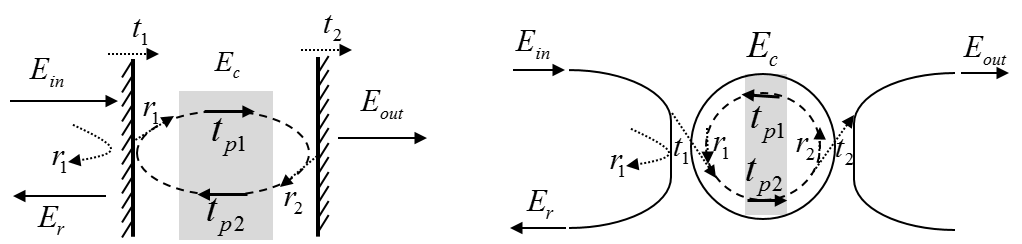
\includegraphics[width=1.0\textwidth]{figures/resonator_v4}
\caption{The ring resonator (right) reflects part of the light incident on the coupler ($r_1$), in the same way that a  mirror reflects $r_1$ field in a Fabry Perot (left). The field inside the cavity ($E_c$) depends on the propagation loss per pass inside the cavity  ($t_{p1}$, $t_{p2}$)  together with
the transmission ($t_1$, $t_2$) and reflection ($r_1$, $r_2$) of the couplers.}
\label{fig:resonator}
\end{figure}
% Resonant cavity schematic: etalon (left), ring (right). 
% For the ring, the transmission port (through) is equivalent to the etalon reflection ($E_r$).


\begin{figure}[htbp]
\centering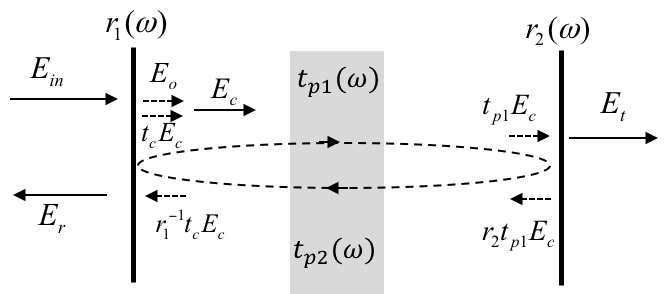
\includegraphics[width=0.8\textwidth]{figures/fp_v6}
\caption{The round trip field transmission of a Fabry-Perot cavity ($t_c$) combines the propagation loss ($t_p =  t_{p1}t_{p2}$) and the loss in the couplers (which act as mirrors) $r_1$ and $r_2$.}
\label{fig:fp}
\end{figure}


The input mirror for the etalon resonator has a power reflectivity of $R_1$ and  transmits or couples $T_1$   of the incident power into the cavity.  For this analysis we assume lossless mirrors so $R_1 + T_1 = 1$.  Some useful relationships for these parameters are

\begin{equation}
R_1 = e^{-\delta_1}
\end{equation}

\begin{equation}
    r_1 = \sqrt{R_1} \hspace{35pt} t_1 = \sqrt{T_1}  
\end{equation}
 
The delta notation $\delta$ follows the formalism provided in the textbook "Lasers" by Siegman \cite{Siegman1986} to describe the round-trip cavity losses. 
The parameters $r_1$ and $t_1$ in Fig.~\ref{fig:fp} simplify the analysis that requires summing up electric fields.
For low-loss cavities the parameter $\delta_1$ can be thought of the coupling coefficient into the cavity (i.e. $   \delta_1 \approx T_1 = \kappa_1$).    


An important parameter in analyzing resonators is the transmission loss after one round trip within the cavity.   To describe this we introduce the round trip electric field transmission coefficient $t_c (\omega)$  which is a complex value given by:

\begin{equation}
  t_c (\omega) = \frac{E_{n+1}}{E_n}  = r_1(\omega) t_{p1}(\omega) t_{p2}(\omega)r_2(\omega) \approx r_1 t_{p1} t_{p2} r_2 e^{-j\theta}
\label{equ:tc}
\end{equation}

\noindent In general, all the reflectivity and transmission parameters can be complex functions of frequency but for  simplicity we will assume they are constants and assume that the only phase variations are due to propagation around the cavity. The propagation transmission parameters $t_{p1}$ and $t_{p2}$ are introduced to deal with ring cavities with asymmetrically located input and output couplers. But for simplicity we will combine them to into a single parameter $t_p = t_{p1} t_{p2}$ to describe the total round trip transmission due to  propagation losses.  The total power transmission due to just propagation losses can then be expressed as
\begin{equation}
T_p = t_p^2 = e^{-\delta_{p}}= e^{-\alpha_p L_c}  
\end{equation}

\noindent which includes both absorption and scattering losses. The parameter $\alpha_p$  is the propagation constant and $L_c$ is the round trip cavity length.    The value $\delta_{p}$  approximates the fractional propagation losses for one round trip cavity circulation.  The phase angle in Eq. (\ref{equ:tc}) depends on the optical frequency  to center frequency difference ($ \nu - \nu_0 $) and free-spectral-range (FSR)

\begin{equation} 
\theta = 2\pi \frac{(\nu - \nu_o)}{FSR}  
\end{equation}  

\noindent where the free-spectral-range of the cavity is given by

\begin{equation} 
FSR = \frac{1}{\tau_c}  = \frac{c}{n_g L_c}
\end{equation}  

\noindent   where  $n_g$ is the average group index and $\tau_c$ is the propagation delay for one round trip in the cavity \cite{Shi:07}. For small cavities it is sometimes preferable to use the round trip cavity delay $\tau_c$ since the FSR becomes large and can be difficult to measure. 

The total power transmission after one complete round trip in the cavity is given by:

\begin{equation}
  T_c = |t_c|^2 = R_1 R_2 T_p  = e^{-\delta_1} e^{-\delta_2} e^{-\delta_p} = e^{-\delta_c}
\end{equation}



\begin{equation} 
  \delta_c = \delta_1 + \delta_2 + \delta_p 
\end{equation} 

\noindent  This simple summing method can be easier than the multiplications  required in the preceding equation.  Often in other analysis approaches these round trip loss parameters are normalized into loss per unit length using the general relationship $\delta = \alpha L_c $.  This can sometimes be counter intuitive when the cavity loss for a discrete coupler or mirror is expressed as a loss per unit length around the cavity.   For low-loss cavities the round trip loss parameter $\delta_c$ can be related to  the Finesse of the cavity by 

\begin{equation} 
F = \frac{FSR}{\Delta\nu}  \approx \frac{2\pi}{\delta_c} 
\label{eq:F}
\end{equation}  

\noindent where $\Delta\nu$ is the full-width-half-maximum width of the resonant peak.
For a cavity loss of $ \delta_c = 1 \space (F \approx 6.28) $ the error in the above finesse approximation is only about 1 percent.


The electric field coupling into and out of the cavity can be expressed as
\begin{equation} E_0 = j t_1 E_{in} \end{equation}
\begin{equation} E_{t} = j t_2 t_{p1} E_c \end{equation}

\noindent      where $E_{in}$ is the incident field, $E_{c}$ is the recirculating resonant field in the cavity and $E_t$ is the output transmitted field.    The relationship between the incident electric field $E_{in}$ and the resonant cavity electric field $E_c$ can be expressed as
\begin{equation} E_c = jt_1E_{in}+t_c(\omega)E_c  \end{equation}  

\noindent  The transfer function for the internal recirculating field inside the resonator can then be written as:

\begin{equation}
\boxed{H_c(\omega) = \frac{E_{c}}{E_{in}} = \frac{jt_1}{1-t_c(\omega)}}      
\label{eq:Hc}
\end{equation}
 
 

The transfer functions for the field transmission ($H_t$) and reflection ($H_r$) are related to the cavity transfer function ($H_c$) by


\begin{equation} 
H_r(\omega) = \frac{E_{r}}{E_{in}} = r_1 + j t_1 t_c r_1^{-1} H_c(\omega) 
\label{eq:Hr}
\end{equation}
\begin{equation} 
H_t(\omega) = \frac{E_{out}}{E_{in}} = j t_2 t_{p1} H_c(\omega)
\label{eq:Ht} 
\end{equation}



\noindent The frequency response for the optical power is obtained by calculating the square of the magnitude of the above field transfer function, for example

\begin{equation} 
\frac{P_{c}}{P_{in}} = \frac{|E_{c}|^2}{|E_{in}|^2}  = |H_c(\omega)|^2
\end{equation}


\section{Complex Lorentzian approximation for high finesse resonators}

In this section we derive simplified analytical expressions for the above cavity transfer functions using the complex Lorentzian approximation.  For Fabry-Perot or Ring resonators with Finesse $F>6$ we can approximate the response centered around the resonance peak using a complex Lorentzian, in the ideal case without backscatter ($R_{bs} = 0$) we can use

\begin{equation}
L(x)  = \frac{1}{1+jx}
\label{eq:Lx}
\end{equation}

\noindent  where

\begin{equation}
x = \frac{2\omega}{\Delta \omega_o} = \frac{2\theta}{\delta_c}
\end{equation}

\noindent  The previous Eqs. (\ref{eq:Hc} -- \ref{eq:Ht}) for the resonator transfer functions can then be simplified to: 

\begin{equation}
H_c = \frac{E_{c}}{E_{in}}  \approx ~ j \frac{ 2~ \sqrt[]{\delta_1}}{\delta_c}  L(x)
\end{equation}

\begin{equation}
H_r = \frac{E_r}{E_{in}} \approx ~ 1 -\frac{2\delta_1}{\delta_c} L(x) 
\label{eq:Hra}
\end{equation}

\begin{equation}
H_t = \frac{E_{out}}{E_{in}} \approx  - \frac{ 2~ \sqrt[]{\delta_1 \delta_2}}{\delta_c}  L(x)
\end{equation}  


\noindent  The approximations ($ R_1 \approx R_2 \approx T_p \approx T_c \approx 1 $) were used where appropriate.
These above approximations can be useful for quickly analyzing experimentally measured frequency responses for high-finesse resonators.
For finesses of $F>15$ the accuracy for the measurable cavity output responses $|H_r(\omega)|^2$ and  $|H_t(\omega)|^2$ are better than $1\%$ using the above complex Lorentzian approximations.  



\section{Measuring resonator losses from reflection response}
In this section we derive some simple analytical expressions to extract the cavity loss parameters from the measured reflectivity from a high-finesse resonator in Fig. \ref{fig:dip}.
The cavity loss can be found from the spectral width of the resonant dip and the input coupling coefficient can be determined by its depth.
Assuming a reasonably low loss resonator ($F>10$) the total cavity loss can be determined by measuring either the finesse or quality factor of the cavity 


\begin{equation} 
\delta_c \approx \frac{2\pi}{F} = \frac{2 \pi m_c}{Q}
\end{equation}

\noindent  where $m_c$ is the cavity mode number which is the round trip cavity group delay normalized by the optical period of the resonant light (i.e.  $m_c = \nu_o \tau_c$ ).



\begin{figure}[htbp]
\centering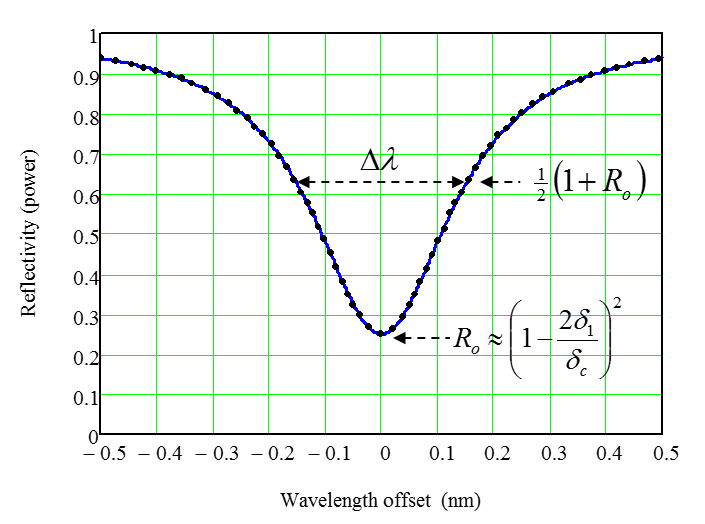
\includegraphics[width=0.7\textwidth]{figures/dip}
\caption{From the resonance width ($ \Delta \lambda $) and depth ($ R_0 $) we extract the cavity loss ($ \delta_c $) and coupling coefficient ($ \delta_1 $), approximating the resonance as a complex Lorentzian and assuming $\alpha_{bs} = 0$.}
\label{fig:dip}
\end{figure}



The measured  reflectivity at resonance ($R_o$)   can be used to estimate the input coupling coefficient ($\delta_1$) and the remaining losses  after the total cavity loss ($\delta_c$) is determined from above.
From Eq. (\ref{eq:Hra}), the resonant dip reflectivity can be approximated by

\begin{equation} 
R_o \approx \Big( 1 -  \frac{2 \delta_1}{\delta_c}       \Big)^2
\end{equation}

\noindent  The input coupling and and other cavity losses can be estimated from

\begin{equation} 
\delta_1 \approx \frac{\delta_c}{2} \big(1 \pm \sqrt{R_0} \big) 
\end{equation}
\begin{equation} 
\delta_p + \delta_2  \approx \frac{\delta_c}{2} \big(1 \mp \sqrt{R_0} \big) 
\end{equation}

\noindent  The $\pm$ sign depends on if the cavity is over or under-coupled. For an over-coupled cavity the input coupling coefficient is larger than half the total cavity losses and for the under-coupled case the input coupling is less than half the total losses. At critical coupling we have  $\delta_1 = \delta_p + \delta_2 = .5\delta_c$  and the resonant dip drops down to zero ($R_o = 0$).  
The above  resonator analysis is accurate with the assumption of zero backscatter in the cavity.  If backscatter is present the peak resonant power can be degraded and the analysis looses its validity.  This can lead to errors when trying to validate models and characterize processing variations based on experimentally estimating coupling coefficients and propagation losses.  To address this problem the below section analyzes the case when backscatter can cause coupling into a reverse direction resonant mode.  



\section{Analysis for backscatter in a resonant cavity}

\begin{figure}[htbp]
\centering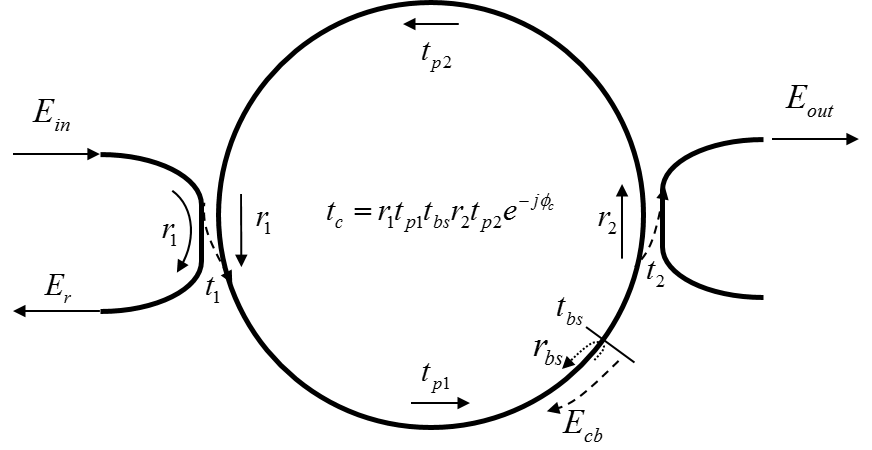
\includegraphics[width=0.8\textwidth]{figures/bs_v3}
\caption{We consider a single reflector (i.e. back-scattering point) to model the two modes that build up inside the cavity.}
\label{fig:bs}
\end{figure}

The analysis in the previous section ignored any backscattering that could couple energy into a backward traveling resonant mode.
When backscattering exists, a backward traveling mode with build up on resonance. 
This backward traveling energy will then couple back into the forward propagating mode (i.e. double backscatter) and affect its resonant properties.
Although backscattering is typically a distributed process throughout the cavity, for a high-Finesse cavity the integrated backscattering can be approximated as a single reflector located within the cavity.
This is valid since the coherence length of the spectrum within the cavity line shape will have a coherence length much longer than the cavity length resulting in a single integrated reflectivity for the multiple scatterers.

For modeling purposes we will introduce a single partially reflective mirror within the waveguide as illustrated in Fig.~\ref{fig:bs} with a power reflectivity $R_{bs}  = r_{bs}^2 = 1-T_{bs}$, where $T_{bs} = t_{bs}^2 = e^{-\delta_{bs}} $.
The analysis will be valid for strong coupling into the backward resonant mode since there is no restriction on the value of $R_{bs}$, but for practical levels of backscattering the assumptions $R_{bs} << 1$ and $T_{bs} \approx 1$ will be used.
Similar to the above analysis the round trip transmission parameters are given by
  
\begin{equation} t_{c}(\omega) = r_1 r_2 t_p t_{bs} e^{-j\theta} \end{equation} 

\begin{equation} 
T_c = |t_c|^2 = R_1 R_2 T_p T_{bs} = e^{-\delta_1} e^{-\delta_2} e^{-\delta_p} e^{-\delta_{bs}} = e^{-\delta_c}  \end{equation}


\begin{equation} 
\delta_c = \delta_1 + \delta_2 + \delta_p + \delta_{bs} \end{equation}  


% The field inside the cavity ($E_c$) relates to the back-scatter ($E_{cb}$):

The total resonant field inside the cavity ($E_c$) now becomes dependent on the back-scattered field ($E_{cb}$) by the following two relationships:

\begin{equation} 
E_c = t_c E_c + jt_1E_{in} + jr_{bs} t_c t_{bs}^{-2} E_{cb} 
\end{equation}  

\begin{equation} 
E_{cb} = t_c E_{cb} + j r_{bs} E_c 
\end{equation}  

These two relationships can be rewritten as  

\begin{equation} E_c = \frac{j t_1 E_{in} + j r_{bs} t_c t_{bs}^{-2} E_{cb} }{1-t_c} \end{equation} 

\begin{equation} E_{cb} = \frac{j r_{bs} E_{c} }{1-t_c} \end{equation} 

The above two Eqs. can now be combined to give the modified transfer function for resonant build up inside the cavity 

\begin{equation} 
\boxed{H_c (\omega) =  \frac{E_c}{E_{in}} = \frac{j t_1 }{(1-t_c)}  \bigg( 1+t_c \Big(\frac{r_{bs} t_{bs}^{-1}}{1-t_c}\Big)^2  \bigg)^{-1}}
\label{eq:Hcbs} 
\end{equation} 

Notice that this result is the same as for the above case with no backscattering except for an additional multiplicative term that goes to unity when the backscatter reflectivity is zero.
This modified transfer function is valid for  large values of $R_{bs}$ since no restrictions were put on this in the model.
Figure \ref{fig:bs_split} illustrates how 3 different levels of backscattering can effect the resonating  power build up in a cavity.
The calculations for the transfer functions  $H_t$ and  $H_r$  remain the same as given in Eqs. (\ref{eq:Ht}) and (\ref{eq:Hr}). It should also be noted that time-domain responses can be obtained by a simple FFT (Fast Fourier Transform) of the frequency-domain results.


It is useful to point the limitations of this simplified model and the result given in Eq. (\ref{eq:Hcbs}).  Experimentally measured resonance splitting will often display asymmetric heights for the two peaks.  It is believed that this asymmetry is due to scattering from the coupler regions or the input and output waveguides that break the symmetry of the above analysis. Due to its increased complexity, this analysis is beyond the scope of this paper.
Although our model assumes a single ring resonator for simplicity, it could easily be extended to coupled resonators (CROWs) \cite{Melloni2010} by making the output coupler frequency dependent ($r_2(\omega)$) to account for the other coupled resonators.

%For high-finesse cavities we can also approximate Eq. (\ref{eq:Hcbs}) using the complex Lorentzian function as defined above in Eq. (\ref{eq:Lx}).

%\begin{equation}
%H_c = \frac{E_{c}}{E_{in}}   \approx    \frac{ j \frac{ 2~ \sqrt[]{\delta_1}}{\delta_c}  L(x)     }{ \big(    1 +  \frac{4 R_{bs}}{\delta^2_c} L^2(x)    \big)    }   \label{eq:Hcbsa}  
%\end{equation}

%Using this approximation we can now estimate the level of backscattering that can be tolerated before significantly effecting the resonating peak power in a cavity.    



\begin{figure}[htbp]
\centering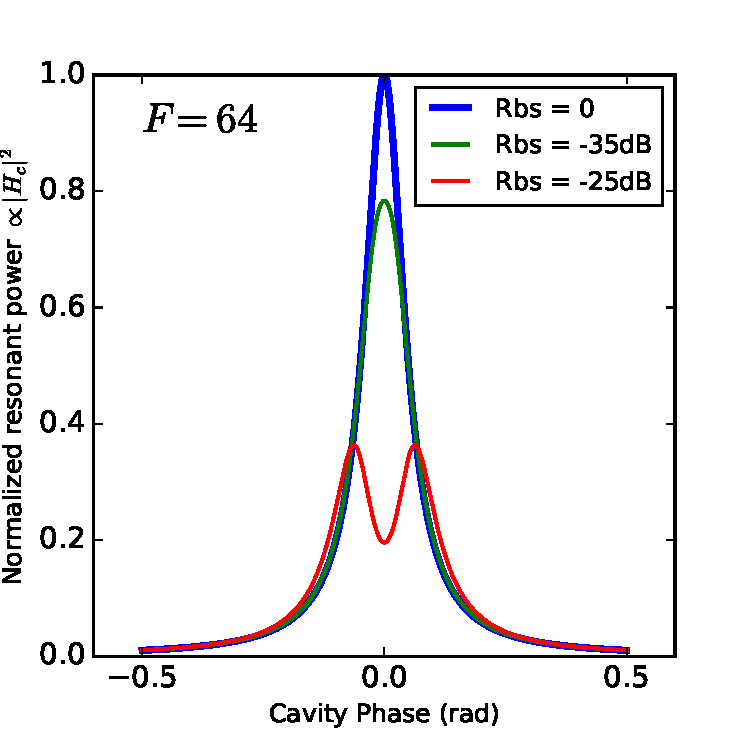
\includegraphics[width=0.6\textwidth]{figures/bs_split.pdf}
\caption{Same ring resonator with different levels of back-scattering (Rbs):
As the back-scatter increases, the forward and backward propagating modes interfere destructively and the resonance splits into two.
F = 64 ($\delta_c = 9.8\%$)} 
\label{fig:bs_split}
\end{figure}
%The coupler couples $T_1 = \kappa_1 = 0.3\%$ into the cavity, which losses total $\Delta_c = 9.8\%$  power.


\section{Conditions when coherent backscatter becomes significant}
We can now examine the correction term in Eq. (\ref{eq:Hcbs}) to determine when the reflectivity $R_{bs}$ becomes large enough to significantly effect the resonating peak power in a cavity.   We will arbitrarily assume that the backscatter becomes important when it causes a drop in the peak internal resonant power by approximately 5\% (0.22~dB).  Referring to Eq. (\ref{eq:Hcbs}) and  converting to optical power using $|H_c|^2$ this equates to an upper bound for $R_{bs}$ given by


\begin{equation}
t_c \Big(\frac{r_{bs} t_{bs}^{-1}}{1-t_c}\Big)^2  \approx \frac{4 R_{bs}}{\delta_c^2} < 0.025  
\end{equation}

\noindent
Recalling that the cavity finesse can be related to the cavity losses by Eq.~(\ref{eq:F}) we get the relatively simple approximation describing  when backscatter reflectivity can be ignored (i.e. less than 5\% drop in peak resonant power) in a low loss cavity

\begin{equation}
R_{bs} < \Big(\frac{1}{2F}\Big)^2
\label{eq:rbs}
\end{equation}
\noindent
As an example to illustrate this result, suppose we consider a series of high-speed ring modulators ($ > 25  Gbps$) for a 16 channel DWDM link.
The required free-spectra-range for each modulator ring might be $ FSR = 16ch \times{100GHz}$ with a resonant spectral width of 25 GHz.
This would equate to a required finesse of approximately  $ F = 64 $   or equivalently a total round trip loss of $ \delta_c = 9.8\% $.
Using the result in Eq. (\ref{eq:rbs}) the backscatter reflectivity should be less than $ R_{bs} < 6.1 \times 10^{-5}  $ or -42 dB.
In addition we can also estimate the required maximum backscattering per unit length for the waveguides in the ring cavity. Assuming a silicon photonics waveguide with group index of about $n_g=4$, the FSR = 1.6 THz corresponds to a round trip cavity length of about 47 microns.
The average value of backscatter should be lower than the above calculated value of -42 dB due to its  random peaking nature from a coherent resonating signal.   For this example we will assume the average backscatter should be 3 times lower than the above peak value estimate.
This would result in a required average value of about $ R_{bs}  = -47 dB  $.
Or expressed differently using the 47 micron cavity length, the waveguide backscatter value should be less than about -34 dB/mm.
This result implies that care should be taken when choosing processing methods for making high-finesse ring cavities since backscattering values of -25 dB/mm have been measured on early e-beam written silicon photonic waveguides \cite{Melati2014a}. 
%[Reference: chapter by Melati et. al. from "Advances in Optics and Photonics, 6, pp. 156-224, 2014.]



\section{Experimental results}
Figure~\ref{fig:bs_measurements} shows measured reflection responses from three test ring resonators made using an e-beam process (see appendix for details).
The original goal was to calibrate the processing results with the design software by experimentally measuring the ring coupling coefficients and waveguide losses.
The experimentally measured solid curves in Fig.~\ref{fig:bs_measurements} illustrate that the random backscatter in each ring can significantly affect the ideal responses predicted by $|H_r(\omega)|^2$ in Eq.~(\ref{eq:Hr}).
To get reasonable fits to the measurement results required using the backscatter modified reflectivity response given by Eqs. (\ref{eq:Hcbs}) and (\ref{eq:Hr}).
The dashed curves in Fig.~\ref{fig:bs_measurements} are obtained by computer fits using the backscatter modified equations.
When compared to computer fits originally performed using the equations without backscatter, differences in the input coupling coefficients could be greater than 20$\%$ and total cavity losses differed by more than 2 times.
This example illustrates that resonator loss parameters can still be estimated even in the presence of waveguide backscattering if an additional fitting variable (i.e. $R_{bs}$) is added to the curve fitting algorithm.  



\label{sec:measurements}

\begin{figure}[htbp]
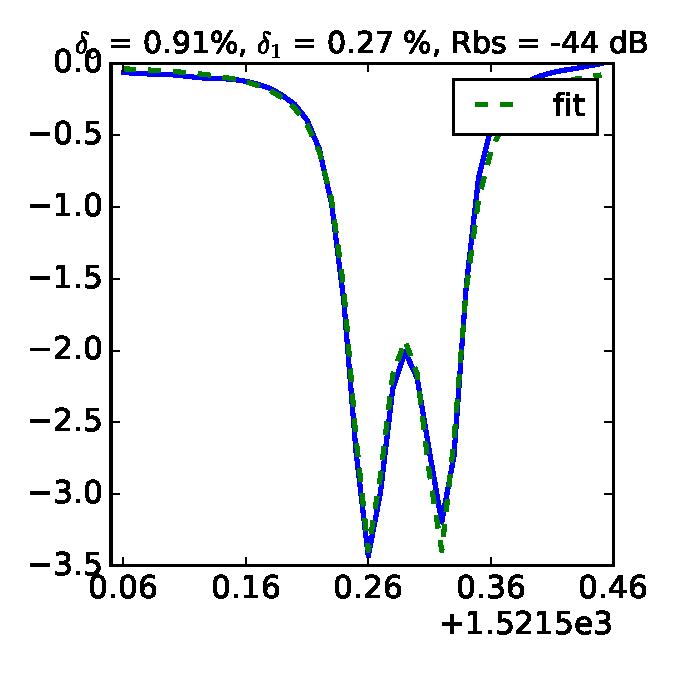
\includegraphics[width=0.32\textwidth]{figures/bs1521.pdf}
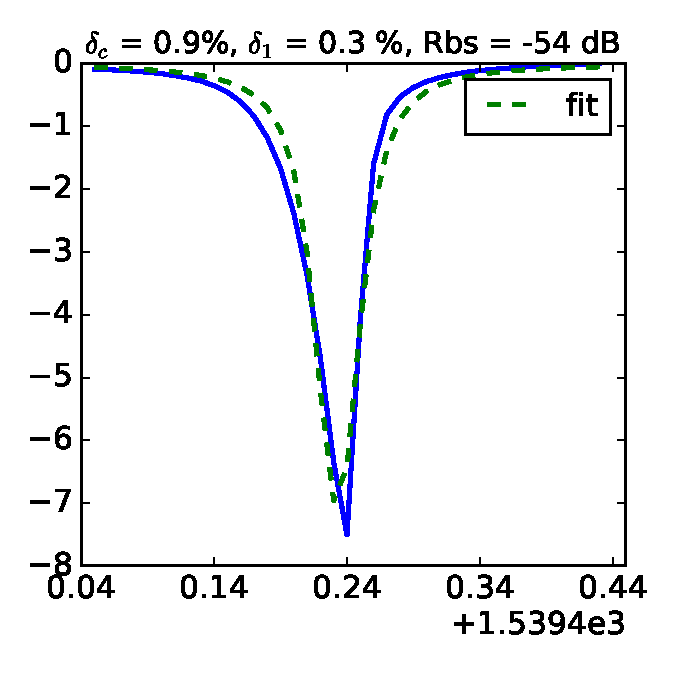
\includegraphics[width=0.32\textwidth]{figures/bs1539.pdf}
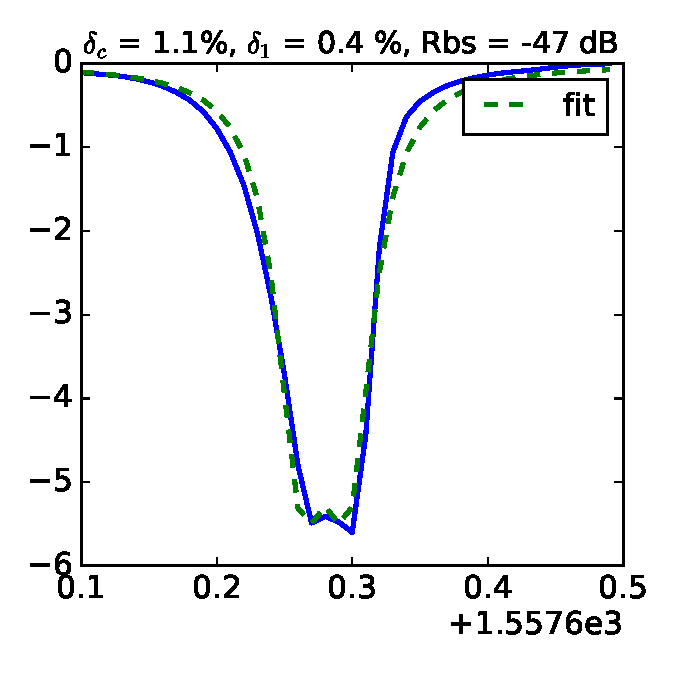
\includegraphics[width=0.32\textwidth]{figures/bs1557.pdf}

\caption{Transmission (dB) versus wavelength (nm) resonances for a $5~\mu m$ radius ring.
Fitting to the back-scatter model  we extract reasonable coupling ($\delta_1$) and cavity loss in the ring ($\delta_c$), while the model without back-scatter would only be valid for resonances lightly affected by back-scatter (middle figure).}
\label{fig:bs_measurements}
\end{figure}


\section{Conclusion}
The presence of backscatter in ring cavities degrades the resonator Q and causes significant mode splitting when reflectivity levels become large.
To model this effect we have derived simple first-order analytical expressions that assume a single backscatterer and match our experimental data.
Using this first order model we also provide a simple relationship based only on the cavity finesse to determine when the backscatter can safely be ignored.
When backscatter can safely be  ignored we also provide simple analytical expressions for quick and simple estimates of the various losses in the cavity.
These simplified expressions can be useful to predict experimental measurements.  


\section*{Appendix: Fabrication}
\label{sec:appendix}
Waveguides were 220~nm height and 500~nm wide. The devices were fabricated using 100 keV Electron Beam Lithography \cite{Bojko2011}. The fabrication used silicon-on-insulator wafer with 220 nm thick silicon on 3$\mu$m thick silicon dioxide. The substrates were 25 mm squares diced from 150 mm wafers. After a solvent rinse and hot-plate dehydration bake, hydrogen silsesquioxane resist (HSQ, Dow-Corning XP-1541-006) was spin-coated at 4000 rpm, then hotplate baked at $80^\circ$C for 4 minutes. Electron beam lithography was performed using a JEOL JBX-6300FS system operated at 100 keV energy, 8 nA beam current, and 500 $\mu m$ exposure field size. The machine grid used for shape placement was 1 nm, while the beam stepping grid, the spacing between dwell points during the shape writing, was 6 nm. An exposure dose of 2800 $\mu C/cm2$ was used. The resist was developed by immersion in 25\% tetramethylammonium hydroxide for 4 minutes, followed by a flowing deionized water rinse for 60 s, an isopropanol rinse for 10 s, and then blown dry with nitrogen. The silicon was removed from unexposed areas using inductively coupled plasma etching in an Oxford Plasmalab System 100, with a chlorine gas flow of 20 sccm, pressure of 12 mT, ICP power of 800 W, bias power of 40 W, and a platen temperature of $20^\circ$C, resulting in a bias voltage of 185 V. During etching, chips were mounted on a 100 mm silicon carrier wafer using perfluoropolyether vacuum oil. 

\section*{Acknowledgments}
We acknowledge edX UBCx Silicon Photonics Design, Fabrication and Data Analysis course supported by the Natural Sciences and Engineering Research Council of Canada (NSERC) and Silicon Electronic-Photonic Integrated Circuits (SiEPIC) program.
Richard Bojko fabricated the devices at the University of Washington Washington Nanofabrication Facility, which is part of the National Science Foundation's National Nanotechnology Infrastructure Network (NNIN).
Zeqin Lu performed the measurements at the University of British Columbia.
We acknowledge Lumerical Solutions, Luceda Photonics (Pierre Wahl, Martin Fiers, Wim Bogaerts and Pieter Dumont) and KLayout for the design software, and professor Lukas Chrostowski for all his help.
\end{document}

